\documentclass{article}
\usepackage[utf8]{inputenc}
\title{vedio 1: RANDOM SAMPLING AND ESTIMATION BIAS}
\author{wbg231 }
\date{December 2022}
\newcommand{\R}{$\mathbb{R}$}
\newcommand{\B}{$\beta$}
\newcommand{\A}{$\alpha$}
\newcommand{\D}{\Delta}

\newcommand{\avector}[2]{(#1_2,\ldots,#1_{#2})}
\newcommand{\makedef}[2]{$\textbf{#1}$:#2 }
\usepackage{tikz,graphicx,hyperref,amsmath,amsfonts,amscd,amssymb,bm,cite,epsfig,epsf,url}

\begin{document}

\maketitle

\section{introduction}
\begin{itemize}
\item \href{https://www.youtube.com/watch?v=iPTTn-hPg_0}{video link}
\section{problem set up}
\item the goal is to estimate  a population parameter
\item for instance we could want to understand the average weight of rats in NYC. in principle we could catch all rats weigh them and find the average
\item so we could chose a subset of the rats find there average weight and use that as an estimate 
\section{estimation a population mean}
\item suppose we are looking at the heights of a population of $N=400$ people
\item Heights: $h_1..H_N$
\item population mean $\mu_{pop}=\frac{1}{N}\Sigma_{i=1}^{N}h_i=175.6$ note that this is a fixed value we want to estimate
\item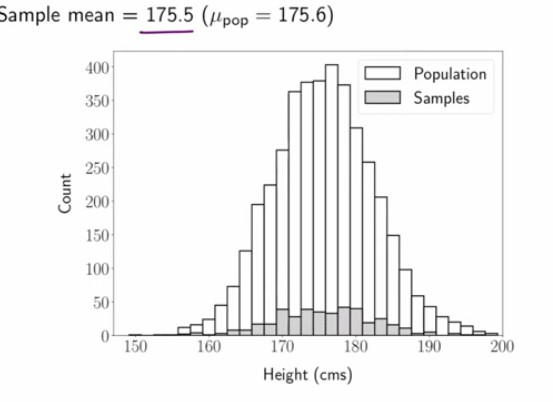
\includegraphics[width=5cm]{notes/week_3/Video-1:RANDOM-SAMPLING-AND-ESTIMATION-BIAS/immages/v1_1.jpg}
\item so just keep in mind that our sample average is a random viable our population parameter is a constant 
\item here is the distribution of the sample mean of size 400 \item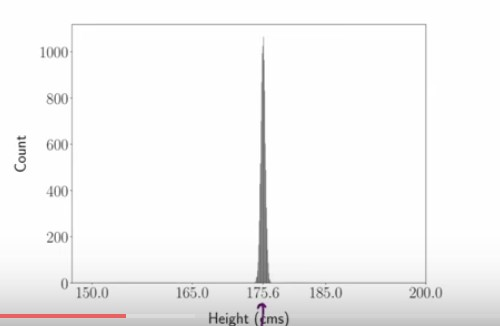
\includegraphics[width=5cm]{notes/week_3/Video-1:RANDOM-SAMPLING-AND-ESTIMATION-BIAS/immages/v2_2.jpg}
\item so know that our sample mean is centered at the population mean and has pretty low variance 
\item this tells us with high probability our estimate will be close to the population parameter 
\section{estimating a population proportion}
\item instead of just getting a population mean we could be interested in a population proportion for instance the proportion of people in NYC with COVID-19 (ie COVID prevalence) call that population proportion $\theta_{pop}=0.05$ the true constant we want to estimate
\item we can try to estimate this with a random sample as well. 
\item as before our random sample proportion is a random variable we are using to estimate a fixed quantity $\theta_{pop}$
\section{random sampling for sample mean}
\item data $a_1...a_n$ this is our fixed data from the population 
\item random sample $\Tilde{x}_1...\Tilde{x_n}$ these are random variables 
\item we assume that each $\Tilde{x}_i$ is selected independently and uniformly at random with replacement (so we could pick someone twice but that will happen with low likely hood in large population)
\item independent means it does not matter who we picked before we pick the next person the same way 
\item uniformly means we have the same likely hood of picking anyone in the population 
\item samples (each $\Tilde{x}_i$) are IID (independent and identically distributed) random variables with pmf $$P_{\Tilde{x}_i}=P(\Tilde{x}_i=a_i)=\frac{1}{n}$$
so note that our random sample is discrete and has equal likely hood of being equal to any individual in our population 
\item here because our data set is random samples our sample average will be a random viable $\Tilde{m}$ such that $$\Tilde{m}=\frac{1}{n}\Sigma_{i=1}^{n}\Tilde{x}_i$$ recall that N is the number of individuals in our population and n is the number of individuals in our sample
\section{random sampling for sample proportion}
\item data $a_1...a_N$ this is our fixed data from the population, where$a_i=1$ if a person meets the condition (ie has COVID) or zero otherwise
\item random sample $\Tilde{x}_1...\Tilde{x_n}$ these are random variables 
\item we assume that each $\Tilde{x}_i$ is selected independently and uniformly at random with replacement (so we could pick someone twice but that will happen with low likely hood in large population)
\item independent means it does not matter who we picked before we pick the next person the same way 
\item uniformly means we have the same likely hood of picking anyone in the population 
\item samples (each $\Tilde{x}_i$) are IID (independent and identically distributed) random variables with pmf $$P_{\Tilde{x}_i}=P(\Tilde{x}_i=a_i)=\frac{1}{n}$$
so note that our random sample is discrete and has equal likely hood of being equal to any individual in our population 
\item here because our data set is random samples our sample proportion  will be a random viable and because the data only takes values zero one our sample proportion will be our sample mean  $\Tilde{m}$ such that $$\Tilde{m}=\frac{1}{n}\Sigma_{i=1}^{n}\Tilde{x}_i$$ recall that N is the number of individuals in our population and n is the number of individuals in our sample
\item so the main point is thees problems are the same 
\section{estimation of population parameters}
\item note we are taking a frequentest perspective, ie we are assume that the parameter of interest is deterministic (this is a choice  as opposed to Bayesian inference) 
\item so we want to think about the probabilistic behavior of the estimator
\section{bias}
\item is the estimator centred at the parameter of interest? 
\subsection{bias definition}
\item for random measurements $\Tilde{x}_1...\Tilde{x}_n$ 
\item and deterministic parameter of interest $\gamma \in \mathbb{R}$
\item and estimator as a function of the random samples $h(\Tilde{x}_1...\Tilde{x}_n)$ 
\item the bias of the estimator is the mean of the error that is $$\text{bias}=E[h(\Tilde{x}_1...\Tilde{x}_n) -\gamma]$$
\item if $E[h(\Tilde{x}_1...\Tilde{x}_n)]=\gamma$ the estimator is unbiased
\item so this is asking is this thing centered?
\subsection{sample mean}
\item what is the mean of the sample mean? $E[\Tilde{m}]=E[\frac{1}{n}\Sigma_{i=1}^{n}\Tilde{x}_{i}]=\frac{1}{n}\Sigma_{i=1}^{n}E[\Tilde{x}_i]$
\item the samples are from the population so $E[\Tilde{x}_i]=\Sigma_{j=1}^{N}a_iP(\Tilde{x}_i=a_{j})=\frac{1}{n}\Sigma_{j=1}^{n}a_j=\frac{1}{n}\Sigma_{j=1}^{N}a_j=\mu_{pop}$
\item so taking this back over we can get $E[\Tilde{m}]=E[\frac{1}{n}\Sigma_{i=1}^{n}\Tilde{x}_{i}]=\frac{1}{n}\Sigma_{i=1}^{n}E[\Tilde{x}_i]=\frac{1}{n}\Sigma_{i=1}^{n}\mu_{pop}=\frac{n}{n}\mu_{pop}=\mu_{pop}$
\item so the take away is that the sample mean is an unbiased estimator of the population mean 
\subsection{sample proportion}
\item recall that the sample proportion is the sample mean ie $\Tilde{m}=\frac{1}{n}\Sigma_{j=1}^{n}\Tilde{x}_j$
\item so we can do a similar argument  $E[\Tilde{x}_j]=\Sigma_{i=1}^{N}a_ip_{\Tilde{x}_j}(a_i)=\Sigma_{i=1}^{N}a_iP(\Tilde{x}_j=a_i)=\frac{1}{N}\Sigma_{i=1}^{N}a_i=\frac{\text{number of covid cases}}{N}$
\item then we can see that 
$E[\Tilde{m}]=E[\frac{1}{n}\Sigma_{j=1}^{n}\Tilde{x}_j]=\frac{1}{n}\Sigma_{j=1}^{n}E[\Tilde{x}_j]=\frac{1}{n}\Sigma_{j=1}^{n}\frac{\text{number of covid cases}}{N}=\frac{\text{number of covid cases}}{N}=\theta_{pop}$ so the population parameter is also unbiased
\item notice that we are assuming that the tests are perfect in this case as well
\item so the fact that the estimator is unbiased is why we observe this behavior with the data centred around the true mean 
\item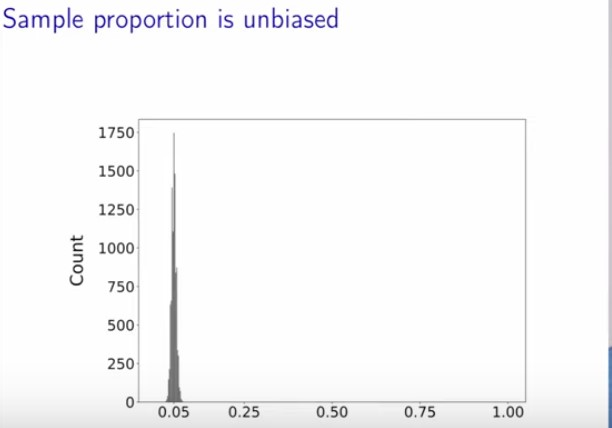
\includegraphics[width=5cm]{notes/week_3/Video-1:RANDOM-SAMPLING-AND-ESTIMATION-BIAS/immages/v1_2.jpg}
\subsection{sample variance}
\item we know that the population mean $\mu_{pop}=\frac{1}{N}\Sigma_{i=1}^{N}a_i$
\item and that the population variance is $\sigma_{pop}^{2}=\frac{1}{N}\Sigma_{i=1}^{N}(a_i-\mu_{pop})^{2}$
\item that is the distance of each value from the population mean 
\item so we can define the sample variance as $$\Tilde{v}=\frac{1}{n-1}\Sigma_{j=1}^{n}(\Tilde{x}_j-\Tilde{m})^{2}$$ (we need to subtract 1 from the denominator to make sure it is unbiased
\item we end up finding that $E[\Tilde{v}]=\sigma_{pop}^{2}$
\item the derivation is kinda pain full. so i am not going to write it out 
\end{itemize}
\end{document}
